\documentclass[12pt]{article}
\usepackage{verbatim}
\usepackage[dvips]{epsfig}
\usepackage{color}
\usepackage{url}
\usepackage[colorlinks=true]{hyperref}

\begin{document}

\section*{GENESIS: Documentation}

{\bf Related Documentation:}
% start: userdocs-tag-replace-items related-do-nothing
% end: userdocs-tag-replace-items related-do-nothing

\section*{De Schutter: Purkinje Cell Model}

\subsection*{Figure\,1}

\begin{figure}[h]
\centering
   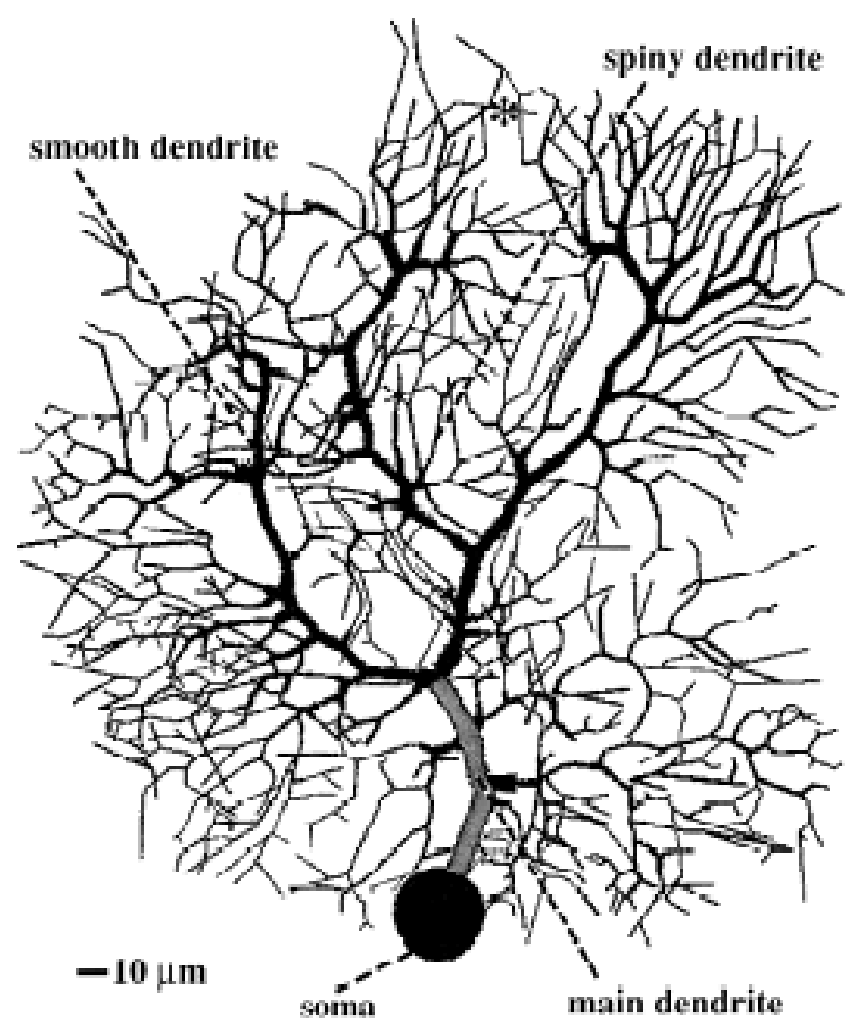
\includegraphics[scale=0.6]{figures/Fig.1.1.eps}
   \caption{Morphology of the Purkinje cell model ({\it cell\,1} of\,\cite{Rapp-P:1994qf}).  The 3 zones with different channel densities (\href{../pub-purkinje-deschutter1-table2/pub-purkinje-deschutter1-table2.tex}{\bf Table\,2}) are marked
as soma (black), main dendrite (dark gray), and the rest of the dendrites
(black). Dashed lines: recording sites displayed in Figs 3-7. Asterisk: recording
site for Figs. 12 and 13.}
   \label{fig:DS1.1}
\end{figure}

\bibliographystyle{plain}
\bibliography{../tex/bib/g3-refs}

\end{document}
